\chapter{Controllo di sistemi MIMO}




\section{Schema di retroazione dell'uscita con integratori}

\begin{equation}
    \begin{cases}
        \dot{x}(t) = Ax(t) + Bu(t) + M d(t) \\
        y(t) = Cx(t) + Nd(t)
    \end{cases}
\end{equation}

L'integratore è necessario per eliminare l'errore a regime,
ora daremo una giustificazione logica di questa affermazione.
Consideriamo che al posto dell'integratore ci sia un blocco \(Z(s)\)
generico come in figura \ref{fig:dim_integratore},
seguiamo il seguente ragionameto:
\begin{enumerate}
    \item Noi vogliamo che l'uscita \(y(t)\) segua un
     riferimento costante \(r(t) = \bar{r}\), quindi vogliamo 
     che a regime valga \(y(t) \to \bar{y} = \bar{r} \), cioè:
    \[\lim_{t \to +\infty} y(t) = \bar{y} = \bar{r}\]
    \item Ma se l'uscita a regime è costante, allora per il teorema del valore finale 
    \item 
    per \(t \to +\infty\) che \(y(t) \to \bar{y} = \bar{r}\).
    \item Ma se \(y(t) \) a regime è costante, allora
    per il teorema del valore finale anche le \(u(t)\) e le \(v(t)\) 
    a regime devono essere costanti.
    \item Inoltre se la \(\bar{y} = \bar{r}\) si ha che a regime l'errore è nullo:
    \[\bar{e} = \lim_{t \to +\infty} e(t) = \lim_{t \to +\infty} r(t) - y(t) = 
    \bar{r} - \bar{y} = 0\]
    \item Ma se l'errore è nullo a regime, allora si ha che in ingresso al blocco 
    \(Z(s)\) si ha un ingresso nullo, quindi il blocco \(Z(s)\) a regime vede un ingresso nullo.
    Quindi il blocco \(Z(s)\) deve essere un integratore, poichè è l'unico operatore che ad 
    un ingresso nullo fornisce in uscita un segnale costante (diverso da zero).
\end{enumerate}

Quindi abbiamo dimostrato che per avere errore nullo a regime il blocco \(Z(s)\)
deve essere proprio un integratore, cioè:
\[Z(s) = \frac{1}{s}\]

\begin{figure}[tbp]
    \centering
    \begin{tikzpicture}[auto, node distance=2cm, >=latex']

        % Stili dei blocchi
        \tikzstyle{block} = [draw, rectangle, minimum height=1cm, minimum width=1cm, align=center]
        \tikzstyle{tallblock} = [draw, rectangle, minimum height=4cm, minimum width=1.5cm, align=center]
        \tikzstyle{sum} = [draw, circle, minimum size=0.6cm, inner sep=0pt, thick]
        \tikzstyle{input} = [coordinate]
        \tikzstyle{output} = [coordinate]
        \tikzstyle{integrator} = [draw, rectangle, minimum height=1cm, minimum width=1cm, align=center]
        % NUOVO STILE per i puntini verticali estesi
        \tikzstyle{vertical dots} = [draw, loosely dotted, very thick, shorten <=3pt, shorten >=3pt]
    
        % --- Riga Superiore (Indice 1) ---
        \node [input] (r1) {};
        \node [sum, right of=r1] (sum1) {};
        % Simbolo di integrale
        \node [integrator, right=1cm of sum1] (int1) {\Large $\displaystyle \int$};
        
        % Etichette segnali riga 1
        \node [above left] at (r1) {$r_1$}; 
        \node at ($(sum1)!0.5!(int1)$) [above] {$e_1$};
        \node at ($(int1.east)+(0.5,0.2)$) {$v_1$}; 
    
        % --- Riga Inferiore (Indice p) ---
        \node [input, below=3cm of r1] (rp) {};
        \node [sum, right of=rp] (sump) {};
        % Simbolo di integrale
        \node [integrator, right=1cm of sump] (intp) {\Large $\displaystyle \int$};
    
        % Etichette segnali riga p
        \node [above left] at (rp) {$r_p$};
        \node at ($(sump)!0.5!(intp)$) [above] {$e_p$};
        
        % --- Blocchi Grandi (K'(s) e G(s)) ---
        \node [tallblock, right=2cm of int1, yshift=-1.5cm] (K) {$K'(s)$};
        \node [tallblock, right=2cm of K] (G) {$G(s)$};
    
        % --- Disturbo d ---
        \draw [->] ($(G.north)+(0,0.8)$) -- (G.north) node[midway, right] {$d$};
    
        % --- Collegamenti Orizzontali ---
        
        % Input r1 -> Sum1
        \draw [->] (r1) -- (sum1) node[pos=0.85, above left] {$+$};
        \draw [->] (sum1) -- (int1);
        \draw [->] (int1) -- (K.west |- int1);
    
        % Input rp -> Sump
        \draw [->] (rp) -- (sump) node[pos=0.85, above left] {$+$};
        \draw [->] (sump) -- (intp);
        \draw [->] (intp) -- (K.west |- intp);
    
        % K'(s) -> G(s)
        \draw [->] (K.east |- int1) -- node[midway, above] {$u_1$} (G.west |- int1);
        \draw [->] (K.east |- intp) -- node[midway, above] {$u_m$} (G.west |- intp);
    
        % G(s) -> Output
        \node [output, right=1.5cm of G.east |- int1] (y1) {};
        \node [output, right=1.5cm of G.east |- intp] (yp) {};
        \draw [->] (G.east |- int1) -- node[near end, above] {$y_1$} (y1);
        \draw [->] (G.east |- intp) -- node[near end, above] {$y_p$} (yp);
    
        % --- PUNTINI VERTICALI ESTESI (Sostituiscono i precedenti) ---
        
        % 1. Sugli Input r
        \draw [vertical dots] (r1) -- (rp);
        
        % 2. Sugli Errori (tra i sommatori)
        \draw [vertical dots] (sum1) -- (sump);
        
        % 3. Tra gli integratori
        \draw [vertical dots] (int1) -- (intp);

        % 4. Zona V (tra Integratore e K) - Calcolo punti medi per allineamento
        \path ($(int1.east)!0.5!(K.west |- int1)$) coordinate (v_mid_top);
        \path ($(intp.east)!0.5!(K.west |- intp)$) coordinate (v_mid_bot);
        \draw [vertical dots] (v_mid_top) -- (v_mid_bot);

        % 5. Zona U (tra K e G)
        \path ($(K.east |- int1)!0.5!(G.west |- int1)$) coordinate (u_mid_top);
        \path ($(K.east |- intp)!0.5!(G.west |- intp)$) coordinate (u_mid_bot);
        \draw [vertical dots] (u_mid_top) -- (u_mid_bot);

        % 6. Sulle uscite y
        \draw [vertical dots] (y1) -- (yp);

        % --- Retroazione ---
        % Loop superiore (alzato per evitare d)
        \draw [->] ($(G.east |- int1)+(0.5,0)$) coordinate (tap1) 
            -- ++(0,1.8) -| (sum1.north) node[pos=0.92, left] {$-$};
    
        % Loop inferiore
        \draw [->] ($(G.east |- intp)+(0.5,0)$) coordinate (tapp) 
            -- ++(0,-1.2) -| (sump.south) node[pos=0.92, left] {$-$};
    
    \end{tikzpicture}
    \caption{Schema di retroazione dell'uscita con integratori}
    \label{fig:control_scheme}
\end{figure}



\begin{figure}[tbp]
    \centering
    \begin{tikzpicture}[auto, node distance=2cm, >=latex']

        % Stili dei blocchi (invariati)
        \tikzstyle{block} = [draw, rectangle, minimum height=1cm, minimum width=1cm, align=center]
        \tikzstyle{tallblock} = [draw, rectangle, minimum height=4cm, minimum width=1.5cm, align=center]
        \tikzstyle{sum} = [draw, circle, minimum size=0.6cm, inner sep=0pt, thick]
        \tikzstyle{input} = [coordinate]
        \tikzstyle{output} = [coordinate]
        \tikzstyle{integrator} = [draw, rectangle, minimum height=1cm, minimum width=1cm, align=center]
        \tikzstyle{vertical dots} = [draw, loosely dotted, very thick, shorten <=3pt, shorten >=3pt]
    
        % --- Riga Superiore (Indice 1) ---
        \node [input] (r1) {};
        \node [sum, right of=r1] (sum1) {};
        % Distanza aumentata a 2cm (già presente)
        \node [integrator, right=2cm of sum1] (int1) {\large $Z(s)$};
        
        % Etichette segnali riga 1
        \node [above left] at (r1) {$r_1 = \bar{r}_{1}$}; 
        \node at ($(sum1)!0.5!(int1)$) [above] {$e_1 = 0$};
        \node at ($(int1.east)+(0.8,0.3)$) {$v_1 = \bar{v}_{1}$}; 
    
        % --- Riga Inferiore (Indice p) ---
        \node [input, below=3cm of r1] (rp) {};
        \node [sum, right of=rp] (sump) {};
        \node [integrator, right=2cm of sump] (intp) {\large $Z(s)$};
    
        % Etichette segnali riga p
        \node [above left] at (rp) {$r_p = \bar{r}_{p}$};
        \node at ($(sump)!0.5!(intp)$) [above] {$e_p = 0$};
        \node at ($(intp.east)+(0.8,0.3)$) {$v_p = \bar{v}_{p}$}; 

        % --- Blocchi Grandi (K'(s) e G(s)) ---
        % MODIFICA IMPORTANTE: Aumentata la distanza da 2cm a 3.5cm
        % Questo allunga la linea di v e sposta i puntini a destra
        \node [tallblock, right=3.5cm of int1, yshift=-1.5cm] (K) {$K'(s)$};
        
        % Aumento leggermente anche lo spazio tra K e G per coerenza
        \node [tallblock, right=2.5cm of K] (G) {$G(s)$};
    
        % --- Disturbo d ---
        \draw [->] ($(G.north)+(0,0.8)$) -- (G.north) node[midway, right] {$d$};
    
        % --- Collegamenti Orizzontali ---
        % Input r1 -> Sum1
        \draw [->] (r1) -- (sum1) node[pos=0.85, above left] {$+$};
        \draw [->] (sum1) -- (int1);
        \draw [->] (int1) -- (K.west |- int1);
    
        % Input rp -> Sump
        \draw [->] (rp) -- (sump) node[pos=0.85, above left] {$+$};
        \draw [->] (sump) -- (intp);
        \draw [->] (intp) -- (K.west |- intp);
    
        % K'(s) -> G(s)
        \draw [->] (K.east |- int1) -- node[midway, above] {$u_1= \bar{u}_{1}$} (G.west |- int1);
        \draw [->] (K.east |- intp) -- node[midway, above] {$u_m = \bar{u}_{m}$} (G.west |- intp);
    
        % G(s) -> Output
        \node [output, right=1.5cm of G.east |- int1] (y1) {};
        \node [output, right=1.5cm of G.east |- intp] (yp) {};
        \draw [->] (G.east |- int1) -- node[near end, above] {$y_1 = \bar{y}_{1}$} (y1);
        \draw [->] (G.east |- intp) -- node[near end, above] {$y_p = \bar{y}_{p}$} (yp);
    
        % --- PUNTINI VERTICALI ESTESI ---
        \draw [vertical dots] (r1) -- (rp);
        \draw [vertical dots] (sum1) -- (sump);
        \draw [vertical dots] (int1) -- (intp);

        % Zona V
        % I puntini si posizionano automaticamente al centro della nuova linea allungata
        \path ($(int1.east)!0.5!(K.west |- int1)$) coordinate (v_mid_top);
        \path ($(intp.east)!0.5!(K.west |- intp)$) coordinate (v_mid_bot);
        \draw [vertical dots] (v_mid_top) -- (v_mid_bot);

        % Zona U
        \path ($(K.east |- int1)!0.5!(G.west |- int1)$) coordinate (u_mid_top);
        \path ($(K.east |- intp)!0.5!(G.west |- intp)$) coordinate (u_mid_bot);
        \draw [vertical dots] (u_mid_top) -- (u_mid_bot);

        % Uscite y
        \draw [vertical dots] (y1) -- (yp);

        % --- Retroazione ---
        \draw [->] ($(G.east |- int1)+(0.5,0)$) coordinate (tap1) 
            -- ++(0,1.8) -| (sum1.north) node[pos=0.92, left] {$-$};
    
        \draw [->] ($(G.east |- intp)+(0.5,0)$) coordinate (tapp) 
            -- ++(0,-1.2) -| (sump.south) node[pos=0.92, left] {$-$};
    
    \end{tikzpicture}
    \caption{Schema per la dimostrazione che l'unico blocco che garantisce errore nullo a 
    regime è l'integratore }
    \label{fig:dimostrazione_integratore}
\end{figure}



Supponiamo ora che il nostro controllore 
\(K'(s)\) 
riesca a stabilizzare il sistema,
cioè che riesca a portare tutti a posizionare 
tutti poli del sistema aumentato 
in retroazione dell'uscita con integratori a sinistra 
dell'asse immaginario (cioè con parte reale negativa).
Supposto questo vogliamo andare a
studiarci le condizioni necessarie affinchè il 
sistema riesca a posizionare 
l'uscita \(y(t)\) al valore di riferimento \(\bar{r}\).
In termine formali vogliamo studiare le condizioni necessarie
affinche a regime si abbia per ogni \(\bar{y}\)
e \(\bar{d}\) (che rappresentano 
rispettivamente il valore di uscita a regime e il disturbo a regime)

\[\begin{cases}
    0 = A \bar{x} + B \bar{u} + M \bar{d} \\
    \bar{y} = C \bar{x} +  N\bar{d}
\end{cases}\]


\begin{equation}
    \begin{pmatrix}
        A & B \\ 
        C & 0 
    \end{pmatrix}
    \begin{pmatrix}
        \bar{x} \\ 
        \bar{u}
    \end{pmatrix} 
    = 
    \begin{pmatrix}
        -M & 0 \\
        -N & I
    \end{pmatrix}
    \begin{pmatrix}
        \bar{d} \\
        \bar{y}
    \end{pmatrix}
\label{sistema_integratori}    
\end{equation}
Questo è un sistema di \(n+p\) equazioni in \(n+m\) ( 
\(\bar{x}\) e \(\bar{u}\) sono incognite ). Definiamo la matrice
\(\Sigma\) come: 
\begin{equation}    
    \Sigma \coloneq \begin{pmatrix}
        A & B \\
        C & 0
    \end{pmatrix} \in \mathbb{R}^{(n+p) \times (n+m)} 
    \label{def_sigma}
\end{equation}
Quello che andremo a fare ora è determinare delle \textbf{condizioni necessarie}
sulla matrice \(\Sigma\) affinchè il sistema 
\eqref{sistema_integratori} ammetta soluzione
\(\forall N\in\mathbb{R}^{p \times r},
M\in\mathbb{R}^{n \times r}, \bar{d}\in \mathbb{R}^{r \times 1} , 
\bar{y}\in\mathbb{R}^{p \times 1}\).
Per determinare queste condizioni necessarie 
andremo a trovare dei casi particolari di \(\Sigma\)
in cui il sistema non ammette soluzione,
dunque condizione necessaria alla soluzione del sistema
è che la matrice \(\Sigma\) non cada in questi casi particolari.\\
Il \textbf{primo caso} particolare che andremo a considerare
è quando il numero di incognite \((n+m)\) del sistema è minore
del numero di equazioni \((n+p)\) del sistema, cioè:
 \begin{equation}
    n + m <  n+p
    \label{eqmagginco}
 \end{equation}
Questo equivale a dire che il numero di colonne della matrice \(\Sigma\)
è minore del numero di righe della matrice \(\Sigma\). Ma questo significa 
che la matrice \(\Sigma\) non può essere di rango pieno per righe
(poichè ha più righe che colonne, ed il rango ha come massimo valore 
dunque il numero di colonne). Se la matrice \(\Sigma\) non è di rango pieno per righe
significa che esistono delle righe della matrice \(\Sigma\) che sono combinazioni lineari delle 
altre righe, dunque facendo delle operazioni elementari sulle righe
(ricordiamo che queste operazioni non cambiano lo spazio delle soluzioni del sistema)
possiamo arrivare rendere nulle queste righe linearmente dipendenti. 
Ma se una riga della matrice \(\Sigma\) è nulla significa che se a 
destra il termine noto assume un valore diverso da zero
il sistema non ammette soluzione. Ma noi vogliamo che il sistema
ammetta soluzione \(\forall N\in\mathbb{R}^{p \times r},
M\in\mathbb{R}^{n \times r}, \bar{d}\in \mathbb{R}^{r \times 1} , 
\bar{y}\in\mathbb{R}^{p \times 1}\), questo significa che
i termini noti possono assumere qualunque valore,
quindi anche un valore diverso da zero. Quindi se scegliamo 
le matrici \(M\) ed \(N\) e i vettori \(\bar{d}\) e \(\bar{y}\)
in modo tale che il termine noto a destra della riga nulla sia diverso 
da zero abbiamo che il sistema non ammette soluzione.  
Dunque abbiamo trovato che nel caso particolare in cui:
\[ n+m < n+p\]
il sistema non ammette soluzione \(\forall N\in\mathbb{R}^{p \times r},
M\in\mathbb{R}^{n \times r}, \bar{d}\in \mathbb{R}^{r \times 1} , 
\bar{y}\in\mathbb{R}^{p \times 1}\). Quindi una condizione necessaria
affinchè il sistema ammetta soluzione è che la condizione 
\eqref{eqmagginco} non sia verificata,
cioè si deve avere:
\[n+m \ge n+p \Longleftrightarrow m \ge p\]
cioè il numero di ingressi deve essere maggiore o uguale
al numero di uscite, cosa che era già intuibile, infatti
se voglio controlla \(p\) uscite dovrò avere un numero di ingressi 
almeno maggiore o uguale a \(p\). Ad esempio se io ho 5 uscite da controllare
almeno dovrò avere 5 ingressi per poter controllare tutte le uscite.\\
Supponiamo ora di aver soddisfatto questa prima condizione necessaria,
cioè di esserci messi nella condizione \(m \geq p\).
Andiamo ora a cercare un \textbf{secondo caso particolare} in cui il sistema
non ammette soluzione. Un'altro caso particolare in cui il sistema
non ammette soluzione è quando il rango della matrice \(\Sigma\)
non è massimo, cioè (poichè siamo nella condizione \(m \geq p\) ):
\[rank(\Sigma) < min\{n+m, n+p\} = n+p\]
Infatti essendo il numero di righe della matrice \(\Sigma\) uguale a \(n+p\),
se il rango della matrice \(\Sigma\) è minore di \(n+p\) significa che esistono
delle righe della matrice \(\Sigma\) che sono combinazioni lineari delle altre righe,
dunque come prima facendo delle operazioni elementari sulle righe
(possibili perchè non cambiano lo spazio delle soluzioni del sistema)
possiamo arrivare rendere nulle queste righe linearmente dipendenti,
e mettendo a destra del sistema il termine noto diverso da zero arriviamo ad un sistema
che non ammette soluzione. Dunque abbiamo trovato un'altro caso particolare
in cui il sistema non ammette soluzione \(\forall N\in\mathbb{R}^{p \times r},
M\in\mathbb{R}^{n \times r}, \bar{d}\in \mathbb{R}^{r \times 1} , 
\bar{y}\in\mathbb{R}^{p \times 1}\). Dunque affinche il sistema ammetta soluzione
sicuramente dobbiamo evitare questo caso particolare, cioè dobbiamo fare in modo che
il rango di \(\Sigma\) sia massimo, cioè dobbiamo avere:
\[rank(\Sigma) = n+p\] 
Quindi le \textbf{ condizioni necessarie} affinche il sistema ammetta soluzione
\(\forall N\in\mathbb{R}^{p \times r},
M\in\mathbb{R}^{n \times r}, \bar{d}\in \mathbb{R}^{r \times 1} , 
\bar{y}\in\mathbb{R}^{p \times 1}\)
\begin{enumerate}
    \item[1)] Il numero di ingressi deve essere maggiore o uguale al numero di uscite:
    \begin{equation}
        m \geq p
    \end{equation}
    \item[2)] La matrice \(\Sigma\) deve essere di rango pieno:
    \begin{equation}
        rank(\Sigma) = min\left\{n+m, n+p\right\} = n+p
        \label{rango_pieno_sigma}
    \end{equation}
\end{enumerate}
La condizione \eqref{rango_pieno_sigma} si può determinare in un modo più formale 
andando anche a considerare la stabilità del sistema in 
retroazione con integratori 
(cosa che fino ad ora abbiamo supposto).
Questa condizione si può determinare andando a studiare il 
sistema aumentato in retroazione con integratori.
Ricordiamo il vettore di stato del sistema aumentato 
è \(\begin{pmatrix}
    x(t) & v(t)
\end{pmatrix}^{T} \in \mathbb{R}^{(n+p) \times 1}\),
dunque le derivate degli stati valgono:
\[
\begin{cases}
    \dot{x}(t) = Ax(t) + Bu(t) + M d(t) \\
    \dot{v}(t) = e(t) = r(t) - y(t) = 
    r(t) - Cx(t) - Nd(t)
\end{cases}
\]
Prendiamo come uscita del sistema aumentato \(\tilde{y}(t) = v(t)\), dunque
si ha che la rappresentazione in forma matriciale 
del sistema aumentato è:
\[
\begin{cases}
    \begin{pmatrix}
        \dot{x}(t) \\ 
        \dot{v}(t)
    \end{pmatrix}
    = \begin{pmatrix}
        A & 0 \\
        -C & 0
    \end{pmatrix}
    \begin{pmatrix}
        x(t) \\ 
        v(t)
    \end{pmatrix}
    + \begin{pmatrix}
        B \\ 
        0
    \end{pmatrix} u(t)
    + \begin{pmatrix}
        M \\ 
        -N
    \end{pmatrix}
        d(t) \\
    \tilde{y}(t) = \begin{pmatrix}
        0 & I
    \end{pmatrix}
    \begin{pmatrix}
        x(t) \\ 
        v(t)
    \end{pmatrix}
\end{cases}
\]
Definiamo \(\tilde{n}\):
\[ \tilde{n} \coloneq  n+p\]
Dunque definiamo le seguenti matrici:
\[\tilde{A} \coloneq \begin{pmatrix}
    A & 0 \\
    -C & 0
\end{pmatrix}\in \mathbb{R}^{\tilde{n} \times \tilde{n}}, \quad
\tilde{B} \coloneq \begin{pmatrix}
    B \\ 
    0
\end{pmatrix} \in \mathbb{R}^{\tilde{n} \times m}, \quad
\tilde{C} \coloneq \begin{pmatrix}
    0 & I
\end{pmatrix} \in \mathbb{R}^{p \times \tilde{n}}\]
Che hanno gli ovvi significati nel sistema aumentato.
Il nostro obiettivo iniziale era trovare un controllore 
\(K'(s)\) che stabilizzasse il sistema in retroazione con integratori,
cioè che rendesse asintoticamente stabile il sistema aumentato.
Condizione necessaria affinchè esista un controllore \(K'(s)\)
che stabilizzi il sistema aumentato è che il sistema aumentato
sia:
\begin{enumerate}
    \item[1)] Completamente raggiunbile
    \item[2)] Completamente osservabile
\end{enumerate}
Queste due condizioni equivalgono a dire che:
\begin{enumerate}
    \item[1)] La coppia \((\tilde{A} , \tilde{B})\) è completamente raggiunbile
    \item[2)] La coppia \((\tilde{A} , \tilde{C})\) è completamente osservabile
\end{enumerate}
Quindi dobbiamo ora studiarci la raggiungibilità e l'osservabilità
del sistema aumentato. Andiamo prima a studiare l'\textbf{osservabilità},
cioè il rango della matrice di osservabilità
(ricordiamo che affinchè il sistema sia completamente osservabile il rango 
deve essere massimo cioè uguale a \(\tilde{n}\) ):
\begin{figure}[H]
\centering
\begin{tikzpicture}[baseline=(current bounding box.center)]
    % --- STILE ---
    \tikzset{brace_style/.style={decoration={brace, amplitude=6pt, raise=6pt}, decorate, thick}}

    % --- 1. NODO MATRICE (RHS) ---
    % Contiene la colonna di blocchi C, CA, etc.
    \node (matrix_node) [font=\large] {
        $
        \displaystyle
        \begin{pmatrix}
            \tilde{C} \\
            \tilde{C} \tilde{A} \\
            \vdots \\
            \tilde{C} \tilde{A}^{\tilde{n}-1}
        \end{pmatrix}
        $
    };

    % --- 2. NODO EQUAZIONE (LHS) ---
    % Allineato a sinistra della matrice
    \node [anchor=east, font=\large] at (matrix_node.west) {
        $M_{O}(\tilde{A}, \tilde{C}) =$
    };

    % --- 3. DISEGNO GRAFFE ---

    % Graffa SOPRA (ROSSA) - n+p colonne
    \draw [brace_style, red] (matrix_node.north west) -- (matrix_node.north east) 
        node [pos=0.5, above=12pt, red, font=\large] {\footnotesize $n+p$ colonne};

    % Graffa A DESTRA (BLU) - np righe
    \draw [brace_style, blue] (matrix_node.north east) -- (matrix_node.south east) 
        node [pos=0.5, right=12pt, blue, font=\large] {\footnotesize $np$ righe};

\end{tikzpicture}
\end{figure}
Ricordando che \(\tilde{C} = \begin{pmatrix}
    0 & I
\end{pmatrix}\) e 
\(\tilde{C}\tilde{A} = \begin{pmatrix}
    A & 0 \\ 
    -C & 0
\end{pmatrix}\)si ha :

\[\tilde{C}\tilde{A}^{2} = 
\begin{pmatrix}
    0 & I
\end{pmatrix} \begin{pmatrix}
    A & 0 \\ 
    -C & 0
\end{pmatrix} 
\begin{pmatrix}
    A & 0 \\ 
    -C & 0
\end{pmatrix} 
=
\begin{pmatrix}
    0 & I
\end{pmatrix} 
\begin{pmatrix}
    A^{2} & 0 \\ 
    -CA & 0
\end{pmatrix} = 
\begin{pmatrix}
    -CA & 0
\end{pmatrix}\]
L'espressione generale \(\forall k \in \mathbb{N}\) è:
\[\tilde{C}\tilde{A}^{k} =
\begin{pmatrix}
    0 & I
\end{pmatrix} 
\begin{pmatrix}
    A^{k} & 0 \\ 
    -CA^{k-1} & 0
\end{pmatrix}
= 
\begin{pmatrix}
    -CA^{k-1} & 0
\end{pmatrix}
\]
Quindi \(M_{O}(\tilde{A}, \tilde{C})\) si può scrivere come:

\begin{figure}[H]
\centering
\begin{tikzpicture}
    % --- STILE ---
    \tikzset{brace_style/.style={decoration={brace, amplitude=6pt, raise=8pt}, decorate, thick}}

    % --- 1. DEFINIZIONE MATRICE (TikZ Matrix) ---
    \matrix (M) [matrix of math nodes, 
                 left delimiter={(}, 
                 right delimiter={)}, 
                 nodes={anchor=center, font=\large}, 
                 column sep=25pt, 
                 row sep=12pt
                 ] {
        0 & I \\
        -C & 0 \\
        -CA & 0 \\
        \vdots & \vdots \\
        -CA^{n-1} & 0 \\
        \vdots & \vdots \\
        -CA^{\tilde{n}-2} & 0 \\
    };

    % --- 2. NODO EQUAZIONE (LHS) ---
    % Ho aggiunto xshift=-10pt per distanziarlo dalla parentesi sinistra
    \node [anchor=east, xshift=-10pt] at (M.west) { \large $M_{O} (\tilde{A} , \tilde{C}) =$ };

    % --- 3. CALCOLO DEI PUNTI DI DIVISIONE ---
    \coordinate (split_col_X) at ($(M-7-1.east)!0.5!(M-7-2.west)$);
    \coordinate (split_row_Y) at ($(M-1-2.south)!0.5!(M-2-2.north)$);

    % --- PARAMETRO FESSURA GRAFFE ---
    \def\gap{3pt}

    % --- 4. DISEGNO GRAFFE SUPERIORI (ROSSE - COLONNE) ---
    \draw [brace_style, red] (M.north west) -- ([xshift=-\gap] M.north -| split_col_X) 
        node [midway, above=14pt, red] {\footnotesize $n$ colonne};

    \draw [brace_style, red] ([xshift=\gap] M.north -| split_col_X) -- (M.north east) 
        node [midway, above=14pt, red] {\footnotesize $p$ colonne};

    % --- 5. DISEGNO GRAFFE LATERALI (BLU - RIGHE) ---
    \draw [brace_style, blue] (M.north east) -- ([yshift=\gap] M.east |- split_row_Y) 
        node [midway, right=14pt, blue] {\footnotesize $p$ righe};

    \draw [brace_style, blue] ([yshift=-\gap] M.east |- split_row_Y) -- (M.south east) 
        node [midway, right=14pt, blue] {\footnotesize $(n-1)p$ righe};

\end{tikzpicture}
\end{figure}

Come si può vedere la matrice \(M_{O} (\tilde{A} , \tilde{C}) \)
ha rango pieno \(rank(M_{O}(\tilde{A}, \tilde{C}) ) = n+p \)
se e solo se la sottomatrice
composta dalle seguenti righe:
\begin{equation}
    \begin{pmatrix}
        -C \\
        -CA\\
        \vdots\\
        -CA^{n-1} \\
        \vdots   \\
        -CA^{\tilde{n}-2} 
    \end{pmatrix} 
    \label{rango_max}    
\end{equation}
ha rango pieno, cioè ha rango \(n\). Ricordiamo
che il rango è limitato superiormente dal minimo
tra il numero
di righe \((np)\) e
il numero di colonne \((n)\), 
quindi in questo caso il limite superiore è dato dal 
numero di colonne. Ora notiamo
che le righe aggiunte dopo la riga \(n\) (quella corrispondente a
\(-CA^{n-1}\)) 
sono linearmente dipendenti
dalle prime \(n\) righe per il teorema di Cayley-Hamilton,
quindi per andare a studiare il rango della matrice
possiamo limitarci a studiare il rango delle righe:
\begin{equation}
    \begin{pmatrix}
        -C \\
        -CA\\
        \vdots\\
        -CA^{n-1} \\
    \end{pmatrix}
    \label{rango_max_lin_ind}
\end{equation}
Affinche la matrice \eqref{rango_max}
abbiamo rango massimo (\(n\)) dobbiamo avere 
che le righe in \eqref{rango_max_lin_ind}
siano linearmente indipendenti, cioè dobbiamo avere che la
matrice \eqref{rango_max_lin_ind} abbia rango \(n\).
Ma questa condizione è proprio la condizione di completa 
osservabilità della coppia \((A,C)\) del sistema 
originale. Quindi il sistema aumentato è completamente osservabile
se e solo se il sistema originale è completamente osservabile.\\
Andiamo ora a studiarci la \textbf{raggiungibilità} 
del sistema aumentato, cioè il rango della matrice di raggiungibilità
(ricordiamo che affinchè il sistema sia completamente raggiungibile
il rango deve essere massimo cioè uguale a \(\tilde{n}\) ):

\begin{figure}[H]
\centering
\begin{tikzpicture}[baseline=(current bounding box.center)]
    % --- STILE ---
    \tikzset{brace_style/.style={decoration={brace, amplitude=6pt, raise=6pt}, decorate, thick}}

    % --- 1. NODO MATRICE (RHS) ---
    \node (matrix_node) [font=\large] {
        $
        \displaystyle
        \begin{pmatrix}
            \tilde{B} & \tilde{A} \tilde{B} & \ldots & \tilde{A}^{\tilde{n}-1} \tilde{B}
        \end{pmatrix}
        $
    };

    % --- 2. NODO EQUAZIONE (LHS) ---
    \node [anchor=east, font=\large] at (matrix_node.west) {
        $M_{R} (\tilde{A} , \tilde{B}) =$
    };

    % --- 3. DISEGNO GRAFFE ---

    % Graffa SOPRA (ROSSA) - colonne
    \draw [brace_style, red] (matrix_node.north west) -- (matrix_node.north east) 
        node [pos=0.5, above=12pt, red, font=\large] {\footnotesize $\tilde{n}m$ colonne};

    % Graffa A DESTRA (BLU) - righe
    \draw [brace_style, blue] (matrix_node.north east) -- (matrix_node.south east) 
        node [pos=0.5, right=12pt, blue, font=\large] {\footnotesize $n+p$ righe};

\end{tikzpicture}
\end{figure}

L'espressione generale \(\forall k \in \mathbb{N}\) è:
\[\tilde{A}^{k}\tilde{B} = 
\begin{pmatrix}
    A^{k} & 0 \\ 
    -CA^{k-1} & 0
\end{pmatrix}
\begin{pmatrix}
    B \\ 
    0
\end{pmatrix}
= 
\begin{pmatrix}
    A^{k}B \\ 
    -CA^{k-1}B
\end{pmatrix}
\]
Quindi la matrice di raggiungibilità del sistema aumentato si può scrivere come:

\begin{figure}[H]
    \centering
    \begin{equation} \label{eq:matrix_MR}
    \begin{tikzpicture}[
        % Allinea la baseline dell'intera figura con la baseline del nodo "EqNode" (l'equazione)
        baseline=(EqNode.base),
        % Stile base generico
        bracebase/.style={decorate, thick},
        % Stile ROSSO PICCOLO: raise standard
        redbrace/.style={bracebase, red, decoration={brace, amplitude=6pt, raise=6pt}},
        % Stile ROSSO GRANDE: aumentato raise per evitare collisioni con i font più grandi
        grandbrace/.style={bracebase, red, decoration={brace, amplitude=10pt, raise=38pt}},
        % Stile BLU: raise standard
        bluebrace/.style={bracebase, blue, decoration={brace, amplitude=6pt, raise=18pt}},
        % Stile per la matrice: aggiunto font=\large e aumentata la spaziatura celle
        mymatrix/.style={matrix of math nodes, left delimiter=(, right delimiter=), 
                         nodes={inner sep=5pt, font=\large}, 
                         row sep=15pt, column sep=18pt, 
                         ampersand replacement=\&}
    ]

    % Definizione della matrice
    \matrix (M) [mymatrix] {
        B \& AB \& A^{2}B \& \cdots \& A^{\tilde{n}-1}B \\
        0 \& -CB \& -C A B \& \cdots \& -C A^{\tilde{n}-2} B \\
    };

    % Etichetta dell'equazione a sinistra
    % Aumentato xshift a -15pt per distanziare l'uguale dalla parentesi
    \node (EqNode) [anchor=east, xshift=-15pt] at (M.west) {$M_{R}(\tilde{A},\tilde{C}) = \null$};

    % --- Annotazioni Orizzontali (ROSSE PICCOLE) ---
    \foreach \col in {1,2,3,5} {
         \draw [redbrace] (M-1-\col.north west) -- (M-1-\col.north east)
            node [midway, above=12pt, red] {$m$};
    }

    % --- Annotazione Orizzontale (ROSSA GRANDE - Totale) ---
    % Aumentato 'above' a 50pt per scavalcare le etichette sottostanti
    \draw [grandbrace] (M-1-1.north west) -- (M-1-5.north east)
        node [midway, above=50pt, red] { $\tilde{n}m$};

    % --- Annotazioni Verticali (BLU) ---
    \coordinate (Split) at ($(M-1-5.south)!0.5!(M-2-5.north)$);
    
    % Graffa blu per la prima riga (n)
    \draw [bluebrace] (M.north east) -- (M.north east |- Split) 
        node [midway, right=25pt, blue] {$n$};

    % Graffa blu per la seconda riga (p)
    \draw [bluebrace] (M.north east |- Split) -- (M.south east) 
        node [midway, right=25pt, blue] {$p$};

    \end{tikzpicture}
    \end{equation}
\end{figure}
Andiamo ora ad enunciare il seguente lemma che lega la raggiungibilità
del sistema aumentato con la raggiungibilità del sistema originale.

\begin{lemma}\label{necc_orig_compl_ragg}
Se il sistema aumentato è completamente raggiungibile
allora il sistema originale è completamente raggiungibile.
\end{lemma}

\begin{proof}
Noi abbiamo supposto che il sistema aumentato sia completamente raggiungibile,
cioè che la matrice di raggiungibilità del sistema aumentato abbia rango pieno.
Notiamo che la matrice di raggiungibilità del sistema aumentato ha \(n+p\)
righe dunque per essere di rango pieno deve avere rango \(n+p\):
\[rank(M_{R}(\tilde{A}, \tilde{B})) = n+p\]
Questo significa che tutte le righe della matrice di raggiungibilità
devono essere linearmente indipendenti 
(infatti la matrice ha più colonne che righe, dunque il rango massimo è dato
dal numero di righe). In particolare,
 anche le prime \(n\) righe della matrice di raggiungibilità
devono essere linearmente indipendenti, ma questo significa che la
seguente matrice, costituita dalle prime \(n\) righe della matrice di raggiungibilità,
è di rango pieno (cioè ha rango \(n\) ):
\begin{equation}
    \begin{pmatrix}
        B & AB & A^{2}B & \ldots A^{n-1}B & \ldots & A^{\tilde{n}-1}B 
    \end{pmatrix}
    \label{raggiungibilita_A_B}
\end{equation}
Ma le colonne dopo la colonna \(n\)-esima (cioè le colonne da \(n+1\) a \(n+p\) )
sono linearmente dipendenti dalle prime \(n\) colonne
per il teorema di Cayley-Hamilton. Quindi se la matrice \eqref{raggiungibilita_A_B}
è di rango pieno \(n\) significa che le prime \(n\) colonne sono linearmente indipendenti,
ma questo significa che la seguente matrice ha rango pieno \(n\):
\begin{equation}
    \begin{pmatrix}
        B & AB & A^{2}B & \ldots A^{n-1}B 
    \end{pmatrix}
    \label{raggiungibilita_A_B_lin_ind}
\end{equation}
Ma la matrice \eqref{raggiungibilita_A_B_lin_ind} è proprio la matrice di raggiungibilità
del sistema originale \((A,B)\). Dunque abbia dimostrato che
se il sistema aumentato è completamente raggiungibile
allora la matrice di raggiungibilità del sistema originale
è di rango pieno, cioè che il sistema originale è completamente raggiungibile.
\end{proof}
Dunque condizione necessaria affinche il sistema aumentato sia completamente raggiungibile
è che il sistema originale \((A,B)\) sia completamente raggiungibile.\\

Andiamo ora a ricavare di nuovo 
la condizione necessaria \eqref{rango_pieno_sigma} come abbiamo già detto all'inizio.


Per prima cosa notiamo che la matrice di raggiungibilità del sistema aumentato
\eqref{eq:matrix_MR} si può riscrivere come prodotto di matrici:
\begin{equation}
M_{R} (\tilde{A} , \tilde{B}) =
 \begin{pmatrix}
    A & B \\
    -C & 0
\end{pmatrix}
\begin{pmatrix}
    0 & B & AB & \ldots & A^{\tilde{n}-2}B \\
    I & 0 & 0 & \ldots & 0
\end{pmatrix}
\label{matrix_MR_prodotto}
\end{equation}
Definiamo la matrice \(\tilde{\Sigma} \in \mathbb{R}^{(n+p) \times (n+m)}\) come:
\begin{equation}
\tilde{\Sigma} \coloneq \begin{pmatrix}
    A & B \\
    -C & 0
\end{pmatrix}
\label{def_tilde_sigma}
\end{equation}
Notiamo che questa matrice \(\tilde{\Sigma}\) ha lo stesso rango della matrice \(\Sigma\)
definita in \eqref{def_sigma}
Mentre chiamiamo la matrice a destra del prodotto in 
\eqref{matrix_MR_prodotto} come \(Q \in \mathbb{R}^{(n+m) \times \tilde{n}m}\):
\begin{equation}
Q \coloneq \begin{pmatrix}
    0 & B & AB & \ldots & A^{\tilde{n}-2}B \\
    I & 0 & 0 & \ldots & 0
\end{pmatrix}
\label{def_Q}
\end{equation}
Quindi la \(M_{R}(\tilde{A}, \tilde{B})\) si può scrivere come:
\begin{equation}
M_{R} (\tilde{A} , \tilde{B}) = \tilde{\Sigma} Q
\label{matrix_MR_prodotto_simplified}
\end{equation}

Dimostriamo ora per assurdo che se la matrice \(\tilde{\Sigma}\) 
non è di rango pieno allora la matrice di raggiungibilità del sistema aumentato
non è di rango pieno, vogliamo dimostrare che:
\begin{lemma}\label{necc_sigma_rango_pieno}

Se la matrice di raggiungibilità del sistema aumentato
è di rango pieno allora la matrice \(\tilde{\Sigma}\)
è di rango pieno.
\end{lemma}
ogliamo quindi dimostrare che, affinché la matrice di raggiungibilità 
del sistema aumentato sia di rango pieno, è necessario che
\(\tilde{\Sigma}\) sia di rango pieno.
Ora dimostreremo il teorema \ref{necc_sigma_rango_pieno} per assurdo,
cioè dimostreremo che il negato del teorema \ref{necc_sigma_rango_pieno} 
implica una contraddizione. Notiamo che il negato del teorema \ref{necc_sigma_rango_pieno} 
consiste nel provare a dimostrare che se la matrice \(M_{R}(\tilde{A}, \tilde{B})\)
è di rango pieno allora la matrice \(\tilde{\Sigma}\)
non è di rango pieno. 
\begin{proof}
La nostra ipotesi è che la matrice di raggiungibilità del sistema aumentato
sia di rango pieno, cioè che:
\[rank(M_{R}(\tilde{A}, \tilde{B})) = n+p\]
Vogliamo dimostrare, come tesi, che questa ipotesi implica che la matrice \(\tilde{\Sigma}\)
non sia di rango pieno:
\[rank(\tilde{\Sigma}) < n+p\]
Ma per la proprietà del prodotto delle matrici si ha che:
\[rank(M_{R} (\tilde{A} , \tilde{B})) \leq min\{rank(\tilde{\Sigma}) , rank(Q)\}\]
Cioè si ha che:
\[n+p \leq min\{rank(\tilde{\Sigma}) , rank(Q)\}\]
Ma notiamo che a destra il minimo tra i due ranghi è sicuramente minore o uguale
al rango di \(\tilde{\Sigma}\), dunque si ha che:
\[n+p \leq rank(\tilde{\Sigma})\]
Ma noi avevamo supposto all'inizio che la matrice \(\tilde{\Sigma}\)
non fosse di rango pieno, cioè si ha:
\[n+p < n+p\]
Ma questo è un assurdo. Dunque la nostra tesi iniziale deve essere falsa,
cioè se la matrice di raggiungibilità del sistema aumentato
è di rango pieno allora la matrice \(\tilde{\Sigma}\)
è di rango pieno.
\end{proof}

Ora abbiamo dimostrato che affinche il sistema aumentato
sia completamente raggiungibile (che ricordiamo essere 
condizione necessaria e sufficiente, insieme alla 
completa osservabilità, per la risoluzione del problema 
di controllo) è necessario che la matrice \(\tilde{\Sigma}\)
sia di rango pieno, ma questa matrice come abbiamo detto prima ha lo stesso rango
della matrice \(\Sigma\) definita in \eqref{def_sigma}, dunque abbiamo 
ridimostrato la condizione necessaria \eqref{rango_pieno_sigma},
cioè che la matrice \(\Sigma\) deve essere di rango pieno affinche il problema di 
controllo sia risolvibile.
Ora dimostriamo che se la matrice \(\Sigma\) è di rango pieno 
e il sistema originale è completamente raggiungibile allora il sistema aumentato
è completamente raggiungibile.
\begin{lemma}\label{suff_sigma_rango_pieno_ragg}
Se la matrice \(\Sigma\) è di rango pieno e il sistema originale
è completamente raggiungibile allora il sistema aumentato
è completamente raggiungibile.
\end{lemma}
\begin{proof}
    Vogiamo dimostrare che sotto le ipotesi del teorema
    la matrice di raggiungibilità del sistema aumentato 
    è di rango pieno, cioè che:
    \[rank(M_{R}(\tilde{A}, \tilde{B})) = n+p\]
    Per la proprietà del prodotto delle matrici si ha che:
    \[rank(M_{R} (\tilde{A} , \tilde{B})) \leq min\{rank(\tilde{\Sigma}) , rank(Q)\}\]
    Inoltre una nota disugualianza sui ranghi delle matrici dice che (
        \(M_{R}(\tilde{A}, \tilde{B}) = \tilde{\Sigma} Q\)
    ):
    \[rank(M_{R}(\tilde{A}, \tilde{B})) \geq rank(\tilde{\Sigma}) + rank(Q) - (n+m)\]
    Unendo le due disuguaglianze si ha che:
    \begin{equation}    
    rank(\tilde{\Sigma}) + rank(Q) - (n+m) 
    \leq M_{R}(\tilde{A}, \tilde{B}) \leq min\{rank(\tilde{\Sigma}) , rank(Q)\} 
    \label{disu_compl}
    \end{equation}
    Ma per ipotesi la matrice \(\Sigma\) è di rango pieno:
    \[rank(\tilde{\Sigma}) =n+p\]
    Il sistema originale è completamente raggiungibile,
    dunque la matrice \(Q\) anche essa è di rango pieno:
    \[rank(Q) = n+m\]
    Dunque riscrivendo la disugualianza \eqref{disu_compl} si ha:
    \[ (n+p) + (n+m) - (n+m) \leq rank(M_{R}(\tilde{A}, \tilde{B})) \leq min\{n+p , n+m\}\]
    Da cui si ricava (dato che \(m \geq p\) ):
    \[ n+p \leq rank(M_{R}(\tilde{A}, \tilde{B})) \leq n+p\]
    Dunque si deve per forza avere:
    \[ rank(M_{R}(\tilde{A}, \tilde{B})) = n+p\]
    Quindi la matrice di raggiungibilità del sistema aumentato
    è di rango pieno, cioè il sistema aumentato è completamente raggiungibile.
\end{proof}

Uniamo tutti i risultati ottenuti nei lemmi \ref{necc_orig_compl_ragg},
\ref{necc_sigma_rango_pieno},\ref{suff_sigma_rango_pieno_ragg}
    in un unico teorema che consiste in una condizione necessaria e sufficiente.
\begin{teorema}\label{necc_suff_controllo_con_integratori}
    Il sistema aumentato è completamente raggiungibile
    se e solo se il sistema originale è completamente raggiungibile
    e la matrice \(\Sigma\) è di rango pieno.
\end{teorema}

\section{Problema di Mixed Sensitivity Design}

Il nostro obiettivo ora è andare a formulare le seguente specifiche
di progetto:
\begin{itemize}
    \item Stabilità 
    \item Stabilità robusta 
    \item Performance inseguimento/disturbo
    \item Limitazione controllo
\end{itemize}
sulle funzione di sensitività \(S(s)\) e sensitività complementare \(S'(s)\).

\[E(s) = R(s) - Y(s) =  S(s) (R(s) - D(s)) + T(s) N(s)\]
\[U(s) K (s) S(s) \left(R(s) - D(s) - N(s)\right)\]

\begin{figure}[H]
    \centering
    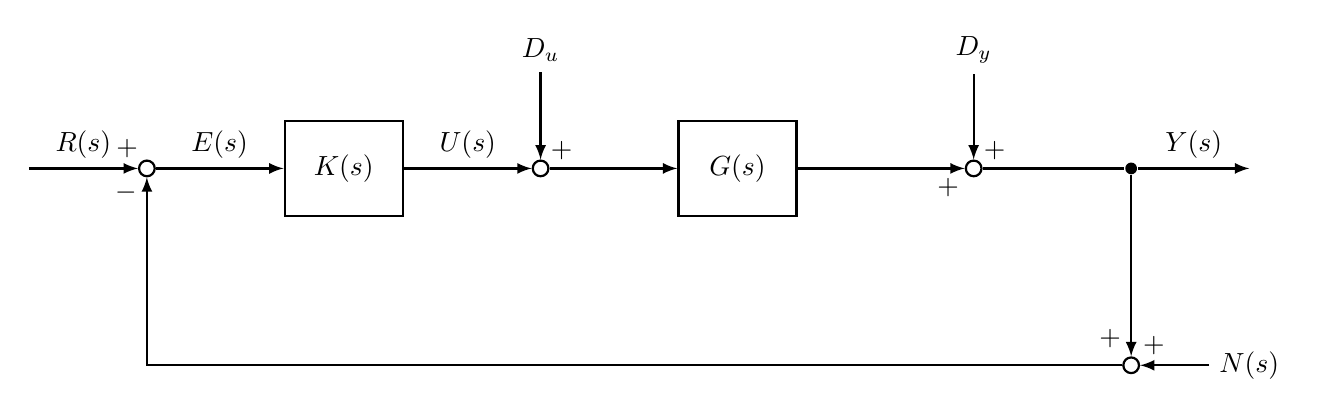
\begin{tikzpicture}[auto, node distance=2cm, >=latex, thick]
        % Stili
        \tikzstyle{block} = [draw, rectangle, minimum height=1.2cm, minimum width=1.5cm, align=center]
        \tikzstyle{sum} = [draw, circle, inner sep=2pt]
        \tikzstyle{coord} = [coordinate]
        \tikzstyle{dot} = [fill=black, circle, inner sep=1.5pt]

        % --- Catena Diretta (Forward Path) ---
        \node [coord] (input) {};
        
        % Sommatore Errore
        \node [sum, right of=input, node distance=1.5cm] (sum1) {};
        
        % Controllore K(s)
        \node [block, right of=sum1, node distance=2.5cm] (controller) {$K(s)$};
        
        % Sommatore Disturbo su U
        \node [sum, right of=controller, node distance=2.5cm] (sum_u) {};
        
        % Processo G(s)
        \node [block, right of=sum_u, node distance=2.5cm] (plant) {$G(s)$};
        
        % Sommatore Disturbo su Y
        \node [sum, right of=plant, node distance=3.0cm] (sum_y) {};
        
        % Punto di prelievo (Measure Point) - Un po' più avanti del sommatore
        \node [dot, right of=sum_y, node distance=2cm] (measure_point) {};
        
        % Uscita finale
        \node [coord, right of=measure_point, node distance=1.5cm] (output) {};

        % --- Nodi per i Disturbi ---
        \node [above of=sum_u, node distance=1.5cm] (du) {$D_u$};
        \node [above of=sum_y, node distance=1.5cm] (dy) {$D_y$};

        % --- Retroazione ---
        % Sommatore per il Rumore N(s) - Allineato verticalmente sotto il punto di prelievo
        \node [sum, below of=measure_point, node distance=2.5cm] (sum_noise) {};
        % Rumore N(s)
        \node [right of=sum_noise, node distance=1.5cm] (noise) {$N(s)$};

        % --- Collegamenti ---
        
        % Ingresso -> Sommatore 1
        \draw [->] (input) -- node {$R(s)$} node[pos=0.9, above] {$+$} (sum1);
        
        % Sommatore 1 -> K(s)
        \draw [->] (sum1) -- node {$E(s)$} (controller);
        
        % K(s) -> Sommatore Du
        \draw [->] (controller) -- node {$U(s)$} (sum_u);
        
        % Disturbo Du -> Sommatore Du
        \draw [->] (du) -- node[pos=0.9, right] {$+$} (sum_u);
        
        % Sommatore Du -> G(s)
        \draw [->] (sum_u) -- (plant);
        
        % G(s) -> Sommatore Dy
        \draw [->] (plant) -- node[pos=0.9, below] {$+$} (sum_y);
        
        % Disturbo Dy -> Sommatore Dy
        \draw [->] (dy) -- node[pos=0.9, right] {$+$} (sum_y);
        
        % Sommatore Dy -> Punto di prelievo -> Uscita
        \draw [->] (sum_y) -- (measure_point) -- node [name=y_out] {$Y(s)$} (output);

        % --- Collegamenti Retroazione ---
        % Scende dal punto di prelievo (measure_point) verso il sommatore del rumore
        \draw [->] (measure_point) -- (sum_noise) node[pos=0.9, left]{ $+$};
        
        % Rumore -> Sommatore Rumore
        \draw [->] (noise) -- (sum_noise) node[pos=0.8, above] {$+$};
        
        % Ritorno al primo sommatore
        \draw [->] (sum_noise) -| (sum1) node[pos=0.96, left] {$-$};

    \end{tikzpicture}
    \caption{Sistema di controllo MIMO con retroazione negativa e disturbi}
    \label{sistema_mimo_retroazione2}
\end{figure}




\begin{equation}
    \begin{cases}
        \| S(s)\|_{\infty} \to 0  \\
        \| T(s)\|_{\infty} \to 0 
    \end{cases}
    \label{norma_infinito_specifiche_iniziali}
\end{equation}

E' impossibile realizzare la condizione precedente poichè 
vale la relazione
\[S(s) + T(s) = I\]
Questo problema si può risolvere ricordando 
che gli ingressi del sistema sono di solito segnali
presenti a frequenze diverse:
\begin{itemize}
    \item Il riferimento \(R(s)\) è a bassa frequenza
    \item Il disturbo \(D(s)\) è a bassa frequenza
    \item Il rumore \(N(s)\) è ad alta frequenza
\end{itemize}

Con queste considerazioni possiamo andare a formulare
le specifiche di progetto in modo diverso, infatti 
le specifiche \ref{norma_infinito_specifiche_iniziali} sono potenti,
ma non necessarie, possiamo accontentarci delle seguenti specifiche, 
più deboli ma sufficienti a soddisfare le nostre esigenze 
(e più che altro realizzabili):
\begin{equation}
    \begin{cases}
        \| S(s)(R(s) - D(s))\|_{2} \to 0, & \forall R,D \textnormal{ reali (cioè stiamo considerando} \\
        & \textnormal{il comportamento frequenziale di } R(s) \textnormal{ e } D(s)) \\[1ex]
        \| T(s) N(s)\|_{2} \to 0, & \forall N \textnormal{ reale (cioè stiamo considerando} \\
        & \textnormal{il comportamento frequenziale di } N(s))
    \end{cases}
    \label{norma-2}
\end{equation}
dove notiamo che \(S(s)(R(s) - D(s))\) e \(T(s) N(s)\)
sono vettori, quindi la norma \(2\) si intende come norma vettoriale.
Infatti se sono vere le \eqref{norma-2} si ha che per la disuguaglianza
triangolare:
\[
\|E(s)\|_{2} \leq \| S(s)(R(s) - D(s))\|_{2} + \| T(s) N(s)\|_{2} \to 0 
\Longrightarrow \|E(s)\|_{2} \to 0
\]
Ma cosa hanno di differente le specifiche \eqref{norma-2} rispetto alle spefiche 
\eqref{norma_infinito_specifiche_iniziali}, la differenza principale sta nel 
fatto che ora possiamo andare ad esplicitare le caratteristiche spettrali
dei segnali \(R(s)\), \(D(s)\) e \(N(s)\), infatti possiamo dire che:
\begin{itemize}
    \item Visto che \(R(s)\) e \(D(s)\) sono segnali a bassa frequenza,
    per soddisfare la prima specifica di \eqref{norma-2} ci basta che \(S(s)\)
    tenda a zero in bassa frequenza, mentre in alta frequenza ci penseranno i segnali 
    \(R(s)\) e \(D(s)\) a far si che la norma vada a zero. Questo si traduce in 
    una specifica sulla norma infinito non più di \(S(s)\) ma di una funzione 
    \(W_{S}(s) S(s)\):
    \[\| W_{S}(s) S(s) \|_{\infty} \to 0\]
    dove \(W_{S}(s)\) è una funzione di peso che ha un valore alto in bassa frequenza
    e un valore basso in alta frequenza, cosichè per soddisfare la specifica
    la funzione \(S(s)\) deve essere piccola in bassa frequenza, come richiesto.
    L'introduzione di questa funzione di peso ci permette di non imporre vincoli in alta 
    frequenza su \(S(s)\), andando quindi a permetterci di imporrre vincoli sulla \(T(s)\),
    continuando però a rispettare l'identità \(S(s) + T(s) = I\).
    Una possibile scelta per \(W_{S}(s)\) per un sistema SISO
     è in Figura \ref{fig:Ws_plot}.
    \item Visto che \(N(s)\) è un segnale ad alta frequenza,
    per soddisfare la seconda specifica di \eqref{norma-2} ci basta che \(T(s)\)
    tenda a zero in alta frequenza, mentre in bassa frequenza ci penserà il segnale
    \(N(s)\) a far si che la norma vada a zero. Questo si traduce in 
    una specifica sulla norma infinito non più di \(T(s)\) ma di una funzione
    \(W_{T}(s) T(s)\):
    \[\| W_{T}(s) T(s) \|_{\infty} \to 0\]
    dove \(W_{T}(s)\) è una funzione di peso che ha un valore basso in bassa frequenza
    e un valore alto in alta frequenza, cosichè per soddisfare la specifica
    la funzione \(T(s)\) deve essere piccola in alta frequenza, mentre in bassa frequenza
    non ci sono vincoli su \(T(s)\), poichè la funzione di peso \(W_{T}(s)\) 
    si occuperà di far andare a zero la norma infinito. 
    Una possibile scelta per \(W_{T}(s)\) per un sistema SISO
     è in Figura \ref{fig:Wt_plot}.
     \item E' possibile definire anche una funzione di peso \(W_{K}(s)\)
     per limitare l'azione di controllo \(U(s)\). Infatti andando 
     a gestire la norma infinito di \(W_{K}(s) K(s) S(s)\):
    \[\| W_{K}(s) K(s) S(s) \|_{\infty} \to 0 \]
    possiamo limitare l'azione di controllo andando a scegliere
    opportunamente la funzione di peso \(W_{K}(s)\). 
    Per un sistema SISO una possibile \(W_{K}(s)\)
    è costante in un largo intervallo di frequenze (quelle 
    possibili per il nostro ingresso di controllo \(U(s)\) ), e va a zero
    in alta frequenza ed in bassa frequenza. Modificando opportunamente il valore costante 
    possiamo andare a limitare l'azione di controllo. Ad esempio aumentando il valore costante
    andremo ad abbassare il valore di \(\left|K(s)S(s)\right|\) (per un sistema SISO 
    \(K(s)S(s)\) è uno scalare e quindi si può parlare di modulo), e di conseguenza 
    andremo ad abbassare il valore di \(\left|U(s)\right|\).
\end{itemize}

Il problema che si occupa di trovare le espressioni delle funzioni di peso 
\(W_{S}(s)\), \(W_{T}(s)\) e \(W_{K}(s)\) prende il nome di 
\textbf{Mixed Sensitivity Design}.

\begin{figure}[tbp]
    \centering
    % --- PRIMA IMMAGINE (SINISTRA): W_S Passa-Basso ---
    \begin{subfigure}[b]{0.48\textwidth}
        \centering
        \begin{tikzpicture}
            \begin{semilogxaxis}[
                width=\linewidth, height=6cm,
                ticks=none,
                axis lines=left,
                xlabel={$\omega$},
                ylabel={$|W_S(j\omega)|_{dB}$},
                xmin=0.01, xmax=1000,
                ymin=-20, ymax=60,
                every axis x label/.style={at={(ticklabel* cs:1)}, anchor=west},
                every axis y label/.style={at={(ticklabel* cs:1)}, anchor=south},
            ]
                \addplot[domain=0.01:1000, samples=300, very thick, black] 
                {20*log10(100 / sqrt(x^2 + 1))};
            \end{semilogxaxis}
        \end{tikzpicture}
        \caption{Funzione peso $W_S(s)$ }
        \label{fig:Ws_plot}
    \end{subfigure}
    \hfill % Spazio tra le due figure
    % --- SECONDA IMMAGINE (DESTRA): W_T Passa-Alto ---
    \begin{subfigure}[b]{0.48\textwidth}
        \centering
        \begin{tikzpicture}
            \begin{semilogxaxis}[
                width=\linewidth, height=6cm,
                ticks=none,
                axis lines=left,
                xlabel={$\omega$},
                ylabel={$|W_T(j\omega)|_{dB}$},
                xmin=0.01, xmax=1000,
                ymin=-50, ymax=30,
                every axis x label/.style={at={(ticklabel* cs:1)}, anchor=west},
                every axis y label/.style={at={(ticklabel* cs:1)}, anchor=south},
            ]
                \addplot[domain=0.01:1000, samples=300, very thick, black] 
                {20*log10( 20 * x / sqrt(x^2 + 10^2) )};
            \end{semilogxaxis}
        \end{tikzpicture}
        \caption{Funzione peso $W_T(s)$ }
        \label{fig:Wt_plot}
    \end{subfigure}
    
    \caption{Andamenti tipici delle funzioni peso per sistemi SISO}
    \label{fig:weights_combined}
\end{figure}


Un modo per risolvere questo problema è
risolvere il problema \(H_{\infty}\)





\section{Problema \(H_{\infty}\) in forma standard}

Consideriamo il sistema in Figura \ref{fig:sistema_H_infinito},
questo sistema rappresenta il sistema di base per andare a formulare
il \textbf{problema di controllo
\(H_{\infty}\) in forma standard}. Notiamo che \(w,u,z,y\) possono 
essere vettori.
Andiamo ad analizzare questo sistema, nello specifico notiamo che la 
relazione ingresso uscita del sistema è data da:
\[ 
\begin{pmatrix}
    Z(s)\\
    Y(s)
\end{pmatrix}
=
G(s)
\begin{pmatrix}
    W(s)\\
    U(s)
\end{pmatrix}\]
La matrice di trasferimento \(G(s)\) si può scomporre in quattro sottomatrici:
\[
G(s) = \begin{pmatrix}
    G_{11}(s) & G_{12}(s) \\
    G_{21}(s) & G_{22}(s)
\end{pmatrix}
\]


\begin{figure}[tbp]
    \centering
    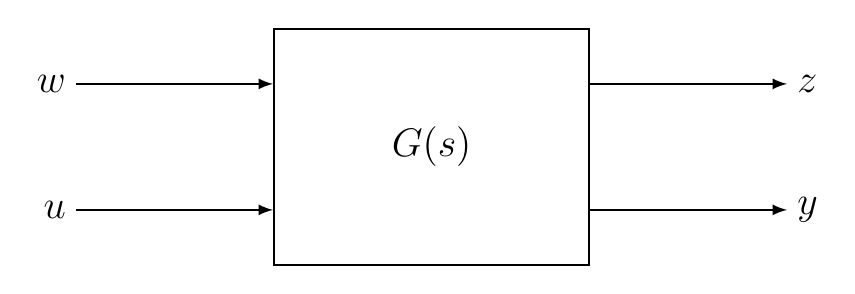
\begin{tikzpicture}[>=latex, thick]
        % Definizione del blocco principale G(s)
        \node[draw, rectangle, minimum width=4cm, minimum height=3cm, align=center] (G) {\Large $G(s)$};

        % Coordinate degli ingressi (lato sinistro)
        % w (sopra) e mu (sotto)
        \draw[->] ([yshift=0.8cm]G.west) +(-2.5,0) node[left] {\Large $w$} -- ([yshift=0.8cm]G.west);
        \draw[->] ([yshift=-0.8cm]G.west) +(-2.5,0) node[left] {\Large $u$} -- ([yshift=-0.8cm]G.west);

        % Coordinate delle uscite (lato destro)
        % z (sopra) e y (sotto)
        \draw[->] ([yshift=0.8cm]G.east) -- +(2.5,0) node[right] {\Large $z$};
        \draw[->] ([yshift=-0.8cm]G.east) -- +(2.5,0) node[right] {\Large $y$};
    \end{tikzpicture}
    \caption{Sistema generale per il controllo \(H_{\infty}\)}
    \label{fig:sistema_H_infinito}
\end{figure}



\begin{figure}[tbp]
    \centering
    \begin{tikzpicture}[>=latex, thick]
        % Blocco principale G(s)
        \node[draw, rectangle, minimum width=4cm, minimum height=2.5cm, align=center] (G) {\Large $G(s)$};

        % Blocco controllore K(s) posizionato sotto
        \node[draw, rectangle, minimum width=2.5cm, minimum height=1.2cm, below=2cm of G] (K) {\Large $K(s)$};

        % Coordinate per gli offset degli ingressi/uscite (superiori e inferiori)
        % yshift positivo per w/z, negativo per mu/y
        
        % Ingresso w (In alto a sinistra)
        \draw[->] ([yshift=0.7cm]G.west) +(-2.5,0) node[left] {\Large $w$} -- ([yshift=0.7cm]G.west);

        % Uscita z (In alto a destra)
        \draw[->] ([yshift=0.7cm]G.east) -- +(2.5,0) node[right] {\Large $z$};

        % Uscita y (In basso a destra) e connessione al feedback
        \draw[->] ([yshift=-0.7cm]G.east) -- +(2.5,0) node[right] {\Large $y$};
        % Ramificazione verso K(s)
        \draw[->] ([yshift=-0.7cm]G.east) ++(1.5,0) |- (K.east);

        % Uscita dal controllore K(s) verso l'ingresso mu (In basso a sinistra)
        % Percorso: Esce da K a sinistra -> va a sinistra -> sale -> entra in G
        \draw[->] (K.west) -| ([xshift=-1.5cm, yshift=-0.7cm]G.west) -- ([yshift=-0.7cm]G.west) node[midway, above] {\Large $u$};

    \end{tikzpicture}
    \caption{Problema di controllo \(H_{\infty}\) in forma standard}
    \label{fig:sistema_H_infinito_feedback}
\end{figure}

Con questa scomposizione si ha che la relazione ingresso uscita
del sistema si può scrivere come:
\begin{equation}
\begin{cases}
        Z(s) = G_{11}(s) W(s) + G_{12}(s) U(s) 
        \\
        Y(s) = G_{21}(s) W(s) + G_{22}(s) U(s) 
\end{cases}
\label{eq:relazione_ingresso_uscita_H_infinito}
\end{equation}
Ora consideriamo il sistema in Figura \ref{fig:sistema_H_infinito_feedback},
dove abbiamo inserito un controllore \(K(s)\) in feedback, si ha:
\[U(s) = K(s)Y(s)\]
Andando a sostituire nel sistema \eqref{eq:relazione_ingresso_uscita_H_infinito}
si ottiene:
\[
\begin{cases}
        Z(s) = G_{11}(s) W(s) + G_{12}(s) Y(s)
        \\
        Y(s) = G_{21}(s) W(s) + G_{22}(s) Y(s)
\end{cases}
\]

Quella che vogliamo andarci a ricavare noi ora è la 
funzione di trasferimento ad anello chiuso tra l'ingresso \(W(s)\)
e l'uscita \(Z(s)\), andiamo quindi a ricavarci \(Y(s)\)
in funzione di \(W(s)\) nella seconda equazione:
\[
\begin{cases}
        Z(s) = G_{11}(s) W(s) + G_{12}(s) Y(s)
        \\
        Y(s) -G_{22}(s) Y(s) = G_{21}(s) W(s)
\end{cases}
\]
Mettendo in evidenza \(Y(s)\) nella seconda equazione si ha:
\[
\begin{cases}
        Z(s) = G_{11}(s) W(s) + G_{12}(s) Y(s)
        \\
        (1 - G_{22}(s))Y(s) = G_{21}(s) W(s)
\end{cases}
\]
Moltiplicando ambo i membri della seconda equazione per
\((1 - G_{22}(s))^{-1}\) si ottiene:
\[
\begin{cases}
        Z(s) = G_{11}(s) W(s) + G_{12}(s) Y(s)
        \\
        Y(s) = (1 - G_{22}(s))^{-1} G_{21}(s) W(s)
\end{cases}
\]
Sostituendo l'espressione di \(Y(s)\) nella prima equazione
si ottiene:
\[ 
Z(s) = G_{11}(s) W(s) + G_{12}(s) (1 - G_{22}(s))^{-1} G_{21}(s) W(s)
\]
Mettendo in evidenza \(W(s)\) si ha:
\[    Z(s) = \left(G_{11}(s) + G_{12}(s) (1 - G_{22}(s))^{-1} G_{21}(s)\right) W(s)\]
Quindi la funzione di trasferimento ad anello chiuso tra l'ingresso \(W(s)\)
e l'uscita \(Z(s)\) è data da:
\begin{equation}
    T_{zw}(s) = G_{11}(s) + G_{12}(s) (1 - G_{22}(s))^{-1} G_{21}(s)
    \label{funzione_trasferimento_H_infinito}
\end{equation}
Ora siamo in grado di formulare il problema di controllo \(H_{\infty}\)
su un sistema in forma standard come quello in Figura \ref{fig:sistema_H_infinito},
che però ha una forma diversa dal nostro sistema in retroazione di uscità.
Nella prossima sezione andremo a vedere come utilizzare i risultati ottenuti per il 
problema di controllo \(H_{\infty}\) in forma standard per risolvere
il problema di mixed sensitivity design.


\section{Problema di 
Mixed Sensitivity come problema \(H_{\infty}\) in forma standard}
Ricordiamo che il nostro schema di retroazione dell'uscita
è quello in Figura \ref{fig:sistema_mimo_retroazione2}, e 
la funzione di cui vogliamo minimizzare la norma infinito
è la seguente:
\[\min_{K(s)}
\left\|
\begin{pmatrix}
    W_{S}(s) S(s) \\
    W_{T}(s) T(s) \\
    W_{K}(s) K(s) S(s)
\end{pmatrix}
\right\|_{\infty}
\]
Ma se riuscissimo a portare il sistema in Figura \ref{fig:sistema_mimo_retroazione2}
nella forma del sistema in Figura \ref{fig:sistema_H_infinito}
in modo tale che la funzione di trasferimento \(T_{zw}(s)\)
sia uguale a:
\[
T_{zw}(s) = 
\begin{pmatrix}
    W_{S}(s) S(s) \\
    W_{T}(s) T(s) \\
    W_{K}(s) K(s) S(s)
\end{pmatrix}
\]
allora potremmo tradurre la risoluzione del problema di mixed sensitivity
design in un problema di controllo \(H_{\infty}\) in forma standard.
Ora andremo a costruirci un sistema fittizio a partire dal sistema in Figura 
\ref{fig:sistema_mimo_retroazione2} in modo tale che sia equivalente 
al sistema in Figura \ref{fig:sistema_H_infinito} e con una funzione di trasferimento
\(T_{zw}(s)\) uguale a quella desiderata.
Il sistema fittizio è mostrato in Figura \ref{fig:sistema_mimo_retroazione_H_infinito},
questo sistema ha come ingressi i segnali \(w\) e \(u\) e come uscite i segnali
\(z_{1}\), \(z_{2}\), \(z_{3}\) e \(y\). Poniamo \(z\) come:
\[
z = \begin{pmatrix}
    z_{1} \\
    z_{2} \\
    z_{3}
\end{pmatrix}
\]
Ora quello che noi vogliamo andare a trovare è la funzione di trasferimento
\(\bar{G}(s)\) che lega:
\[
\begin{pmatrix}
    Z(s)\\
    Y(s)
\end{pmatrix}
=
\bar{G}(s)
\begin{pmatrix}
    W(s)\\
    U(s)
\end{pmatrix}
\]


\[\bar{G}(s) = \begin{pmatrix}
    G_{11}(s) & G_{12}(s) \\
    G_{21}(s) & G_{22}(s)
\end{pmatrix} 
\]

\[Z_{1}(s) = W_{S}(s) Y(s) = W_{S}(s) \left(W(s) - G(s)U(s)\right) \]
\[Z_{2}(s) = W_{K}(s) U(s) \]
\[Z_{3}(s) = W_{T}(s) G(s) U(s)\]


\[\bar{G}(s)= \begin{pmatrix}
    W_{S}(s)  & -W_{S}(s) G(s) \\
    0  & W_{K}(s) \\
    0  & W_{T}(s) G(s) \\
    I & -G(s)
\end{pmatrix}\]



Ora una volta ricavata la funzione di trasferimento \(\bar{G}(s)\),
quello che vogliamo andare a dimostrare è che il nostro problema \(H_{\infty}\)
standard è equivalente al problema di mixed sensitivity design,
cioè che la funzione di trasferimento ad anello chiuso
tra l'ingresso \(W(s)\) e l'uscita \(Z(s)\) sia uguale a:
\[
T_{zw}(s) =
\begin{pmatrix}
    W_{S}(s) S(s) \\
    W_{T}(s) T(s) \\
    W_{K}(s) K(s) S(s)
\end{pmatrix}
\]

\begin{figure}[tbp]
\centering
\begin{tikzpicture}[auto, node distance=2cm, >=latex']
    % Definition of styles
    \tikzstyle{block} = [draw, rectangle, minimum height=2.5em, minimum width=3.5em]
    \tikzstyle{sum} = [draw, circle, inner sep=0pt, minimum size=6mm, node distance=1cm]
    \tikzstyle{input} = [coordinate]
    \tikzstyle{output} = [coordinate]

    % Placement of nodes
    \node [input] (input) {};
    \node [sum, right of=input, node distance=1.5cm] (sum) {};
    \node [block, right of=sum, node distance=2.5cm] (K) {$K(s)$};
    \node [block, right of=K, node distance=3.5cm] (G) {$G(s)$};
    
    % Weights positioned on the right
    % WT (basso)
    \node [block, right of=G, node distance=4cm, yshift=1.2cm] (WT) {$W_T$};
    % WK (medio)
    \node [block, above of=WT, node distance=2cm] (WK) {$W_K$};
    % WS (alto)
    \node [block, above of=WK, node distance=2cm] (WS) {$W_S$};
    
    % Nodes for weight outputs
    \node [output, right of=WT, node distance=1.5cm] (outT) {};
    \node [output, right of=WK, node distance=1.5cm] (outK) {};
    \node [output, right of=WS, node distance=1.5cm] (outS) {};

    % Main Connections
    \draw [->] (input) -- node {$w$} node[pos=1.1, anchor=south east] {$+$} (sum);
    \draw [->] (input) -- node {$w$} (sum);
    \draw [->] (sum) -- node [name=y] {$y$} (K);
    \draw [->] (K) -- node [name=u] {$u$} (G);

    % Connection to WT: Right, then Up, then Right
    \draw [->] (G.east) -- ++(1,0) |- (WT.west);
    
    % Connections to weights WS and WK
    \draw [->] ($(sum)!0.6!(K)$) |- (WS);
    \draw [->] ($(K)!0.6!(G)$) |- (WK);
    
    % Output lines from weights with labels z1, z2, z3 (Top to Bottom)
    \draw [->] (WS) -- node [near end] {$z_1$} (outS);
    \draw [->] (WK) -- node [near end] {$z_2$} (outK);
    \draw [->] (WT) -- node [near end] {$z_3$} (outT);

    % Feedback Loop
    \draw [->] (G.east) ++(0.5,0) -- ++(0,-3.5) -| node[pos=0.96, anchor=south west] {$-$} (sum);

\end{tikzpicture}
\caption{Sistema fittizio per trasformare 
il problema di mixed sensitivity in un problema \(H_{\infty}\) standard. Notiamo 
che la \(y\) non è l'uscita del sistema in retroazione, ma è l'errore 
\(y(t)= e(t)\)}
\label{sistema_mimo_retroazione2}
\end{figure}



La sequenza di passi per andare a formulare e risolvere
un problema di \(H_{\infty}\) standard
è la seguente:
\begin{itemize}
    \item Definizione dell'impianto \(G(s)\)
    \item Traduzione delle specifiche di progetto in termini di funzioni di peso 
    \(W_{S}(s), W_{T}(s), W_{K}(s)\)
    \item Definire \(\bar{G}(s)\) del sistema in forma standard per il problema 
    \(H_{\infty}\)
    \item Risolvere il problema di controllo \(H_{\infty}\)
\end{itemize}


Risolvere il problema di \(H_{\infty}\) ci da un uscita:
\begin{itemize}
    \item Il controllo \(K(s)\)
    \item Un valore \(\gamma >0\) tale che:
    \[\| T_{zw}(s) \|_{\infty} < \gamma \Longrightarrow 
\left\|
\begin{pmatrix}
    W_{S}(s) S(s) \\
    W_{T}(s) T(s) \\
    W_{K}(s) K(s) S(s)
\end{pmatrix}
\right\|_\infty < \gamma
 \]
\end{itemize}
Andiamo a ricordare che noi vogliamo usare il problema \(H_{\infty}\)
per risolvere il problema di mixed sensitivity. Per noi il problema 
di \(H_{\infty}\) associato al problema di mixed sensitivity
è risolto se e solo se \(\gamma < 1\), quindi si ha:
    \[\| T_{zw}(s) \|_{\infty} < 1 \Longrightarrow 
\left\|
\begin{pmatrix}
    W_{S}(s) S(s) \\
    W_{T}(s) T(s) \\
    W_{K}(s) K(s) S(s)
\end{pmatrix}
\right\|_\infty < 1
 \]
\subsection{Costruzione \(W_{S}(s)\)}
Notiamo che le progettazioni sulle funzioni di peso che effettueremo 
ora valgono per sistemi SISO, dunque le funzioni di trasferimento
che andremo a considerare sono tutte funzioni scalari.\\
Ricordiamo che l'errore è dato da:
\[E(s) = S(s) \left(R(s) - D(s)\right) + T(s) N(s)\]

Per quanto riguarda le specifiche sulll'inseguimento del riferimento 
\(R(s)\) le specifiche possibili sono le seguenti:
\begin{itemize}
    \item Errore a regime \(\le \bar{e}_{\infty}\). Ricordiamo che l'errore a regime 
    vale:
    \[e_{\infty} = \lim_{t \to \infty} e(t) = \lim_{s \to 0} s E(s)\]
    se il riferimento è un gradino \(R(s) = \displaystyle 
    \frac{1}{s}\) allora si ha 
    (ricordiamo che stiamo considerando i disturbi nulli \(D(s) = 0\) e \(N(s) = 0\) ):
    \[e_{\infty} = \lim_{t \to \infty} e(t) = \lim_{s \to 0} s E(s) =
    S(0)\]
    Quindi la specifica sull'errore a regime si può riscrivere come:
    \[S(0) \le \bar{e}_{\infty}\]
    Ora il nostro obiettivo è convertire questa specifica su \(S(0)\) in 
    una specifica su \(W_{S}(s)\), in modo tale che se la specifica su \(W_{S}(s)\)
    è soddisfatta allora anche la specifica su \(S(0)\) è soddisfatta.
    Partiamo con il ricordare che per noi il 
    \(H_{\infty}\) associato al problema di mixed sensitivity
    è risolto se e solo se:
    \[\| W_{S}(s) S(s) \|_{\infty} < 1  \]
    Ma per definizione della norma \(H_{\infty}\) si ha che la disugualianza è 
    vera \(\forall s\), quindi in particolare per \(s = 0\):
    \[\left|W_{S}(0)\right| 
    \left|S(0)\right| < 1  
    \Longleftrightarrow \left|S(0)\right| < \frac{1}{\left|W_{S}(0)\right|}\]
    Ora se imponiamo la seguente condizione su \(W_{S}(0)\):
    \[\frac{1}{\left|W_{S}(0)\right|} \le \bar{e}_{\infty}\]
    si il risultato voluto, cioè una specifica su \(W_{S}(s)\) 
    che implica la specifica su \(S(0)\):
    \[\left|S(0)\right| < \frac{1}{\left|W_{S}(0)\right|} \le \bar{e}_{\infty} 
    \Longrightarrow \left|S(0)\right| < \bar{e}_{\infty}\]
    Quindi la specifica sull'errore a regime si può tradurre
    in una specifica su \(W_{S}(0)\):
    \begin{equation}-+    
        \frac{1}{\left|W_{S}(0)\right|} \le \bar{e}_{\infty}  \Longrightarrow 
        \left|W_{S}(0)\right| \ge \frac{1}{\bar{e}_{\infty}}
    \end{equation}
    \item Tempo di assestamento, abbiamo delle specifiche ad esempio
    su \(t_{a5}\) o \(t_{a1}\), ricordiamo:
    \[t_{a5} = 3 \tau  \frac{3}{\omega_{c}}\] 
    \[t_{a1} = 4.6 \tau  \frac{3}{\omega_{c}}\] 
    In letteratura si trova spesso la specifica sul tempo di assestamento 
    espressa come:
    \[t_{a} \approx \frac{4}{\omega_{c}}\]
    Ricordiamo che la frequenza \(\omega_{c}\) è il valore di frequenza
    in cui la \(L(j\omega_{c})\) in \(dB\) ha modulo \(0 dB\), cioè:
    \[\left|L(j\omega_{c})\right|_{dB} = 0 dB \Longleftrightarrow
    \left|L(j\omega_{c})\right| = 1\]
    Questo implica che la funzione di sensitività deve avere:
    \[\left|L(j\omega_{c})\right| = 1 
    \Longrightarrow
    \left|S(j \omega_{c})\right|=\frac{1}{2}\]
    \item Sovraelongazione, che ricordiamo essere legata al 
    modulo di picco della \(S(j\omega)\):
    \[M_{p}\left(S(j\omega)\right) = max_{\omega}
    \left|S(j \omega)\right| \]
    \[\left|W_{S}(j \omega)\right| \textnormal{ in alta frequenza }
    \]
\end{itemize}


\[\| W_{S}(s) S(s)\|_{\infty} < 1 \textnormal{ Disturbi in ingresso}\]
\[\| W_{T}(s) T(s)\|_{\infty} < 1 \textnormal{ Riferimenti in ingresso}\]
Teorema del piccolo guadagno.
\[ \| W_{K}(s) K(s) S(s)\|_{\infty} < 1 \]

\[W_{S} =  \frac{\displaystyle \frac{s}{M_{P}} + \omega_{c}}{s + A \omega_{c}}\]

\begin{itemize}
    \item Fattore di riduzione \(M_{R}\) 
    \item \(\omega_{~}\) di attenuazione
\end{itemize}

\[W_{T} = \displaystyle \frac{\displaystyle \frac{s}{M_{P}} + \omega_{c}}{s + A \omega_{c}}\]

